\PassOptionsToPackage{unicode=true}{hyperref} % options for packages loaded elsewhere
\PassOptionsToPackage{hyphens}{url}
%
\documentclass[11pt,ignorenonframetext,]{beamer}
\usepackage{pgfpages}
\setbeamertemplate{caption}[numbered]
\setbeamertemplate{caption label separator}{: }
\setbeamercolor{caption name}{fg=normal text.fg}
\beamertemplatenavigationsymbolsempty
% Prevent slide breaks in the middle of a paragraph:
\widowpenalties 1 10000
\raggedbottom
\setbeamertemplate{part page}{
\centering
\begin{beamercolorbox}[sep=16pt,center]{part title}
  \usebeamerfont{part title}\insertpart\par
\end{beamercolorbox}
}
\setbeamertemplate{section page}{
\centering
\begin{beamercolorbox}[sep=12pt,center]{part title}
  \usebeamerfont{section title}\insertsection\par
\end{beamercolorbox}
}
\setbeamertemplate{subsection page}{
\centering
\begin{beamercolorbox}[sep=8pt,center]{part title}
  \usebeamerfont{subsection title}\insertsubsection\par
\end{beamercolorbox}
}
\AtBeginPart{
  \frame{\partpage}
}
\AtBeginSection{
  \ifbibliography
  \else
    \frame{\sectionpage}
  \fi
}
\AtBeginSubsection{
  \frame{\subsectionpage}
}
\usepackage{lmodern}
\usepackage{amssymb,amsmath}
\usepackage{ifxetex,ifluatex}
\usepackage{fixltx2e} % provides \textsubscript
\ifnum 0\ifxetex 1\fi\ifluatex 1\fi=0 % if pdftex
  \usepackage[T1]{fontenc}
  \usepackage[utf8]{inputenc}
  \usepackage{textcomp} % provides euro and other symbols
\else % if luatex or xelatex
  \usepackage{unicode-math}
  \defaultfontfeatures{Ligatures=TeX,Scale=MatchLowercase}
\fi
\usetheme[]{metropolis}
% use upquote if available, for straight quotes in verbatim environments
\IfFileExists{upquote.sty}{\usepackage{upquote}}{}
% use microtype if available
\IfFileExists{microtype.sty}{%
\usepackage[]{microtype}
\UseMicrotypeSet[protrusion]{basicmath} % disable protrusion for tt fonts
}{}
\IfFileExists{parskip.sty}{%
\usepackage{parskip}
}{% else
\setlength{\parindent}{0pt}
\setlength{\parskip}{6pt plus 2pt minus 1pt}
}
\usepackage{hyperref}
\hypersetup{
            pdftitle={Lecture 17},
            pdfauthor={Colin Rundel},
            pdfborder={0 0 0},
            breaklinks=true}
\urlstyle{same}  % don't use monospace font for urls
\newif\ifbibliography
\usepackage{color}
\usepackage{fancyvrb}
\newcommand{\VerbBar}{|}
\newcommand{\VERB}{\Verb[commandchars=\\\{\}]}
\DefineVerbatimEnvironment{Highlighting}{Verbatim}{commandchars=\\\{\}}
% Add ',fontsize=\small' for more characters per line
\newenvironment{Shaded}{}{}
\newcommand{\AlertTok}[1]{\textcolor[rgb]{1.00,0.00,0.00}{\textbf{#1}}}
\newcommand{\AnnotationTok}[1]{\textcolor[rgb]{0.38,0.63,0.69}{\textbf{\textit{#1}}}}
\newcommand{\AttributeTok}[1]{\textcolor[rgb]{0.49,0.56,0.16}{#1}}
\newcommand{\BaseNTok}[1]{\textcolor[rgb]{0.25,0.63,0.44}{#1}}
\newcommand{\BuiltInTok}[1]{#1}
\newcommand{\CharTok}[1]{\textcolor[rgb]{0.25,0.44,0.63}{#1}}
\newcommand{\CommentTok}[1]{\textcolor[rgb]{0.38,0.63,0.69}{\textit{#1}}}
\newcommand{\CommentVarTok}[1]{\textcolor[rgb]{0.38,0.63,0.69}{\textbf{\textit{#1}}}}
\newcommand{\ConstantTok}[1]{\textcolor[rgb]{0.53,0.00,0.00}{#1}}
\newcommand{\ControlFlowTok}[1]{\textcolor[rgb]{0.00,0.44,0.13}{\textbf{#1}}}
\newcommand{\DataTypeTok}[1]{\textcolor[rgb]{0.56,0.13,0.00}{#1}}
\newcommand{\DecValTok}[1]{\textcolor[rgb]{0.25,0.63,0.44}{#1}}
\newcommand{\DocumentationTok}[1]{\textcolor[rgb]{0.73,0.13,0.13}{\textit{#1}}}
\newcommand{\ErrorTok}[1]{\textcolor[rgb]{1.00,0.00,0.00}{\textbf{#1}}}
\newcommand{\ExtensionTok}[1]{#1}
\newcommand{\FloatTok}[1]{\textcolor[rgb]{0.25,0.63,0.44}{#1}}
\newcommand{\FunctionTok}[1]{\textcolor[rgb]{0.02,0.16,0.49}{#1}}
\newcommand{\ImportTok}[1]{#1}
\newcommand{\InformationTok}[1]{\textcolor[rgb]{0.38,0.63,0.69}{\textbf{\textit{#1}}}}
\newcommand{\KeywordTok}[1]{\textcolor[rgb]{0.00,0.44,0.13}{\textbf{#1}}}
\newcommand{\NormalTok}[1]{#1}
\newcommand{\OperatorTok}[1]{\textcolor[rgb]{0.40,0.40,0.40}{#1}}
\newcommand{\OtherTok}[1]{\textcolor[rgb]{0.00,0.44,0.13}{#1}}
\newcommand{\PreprocessorTok}[1]{\textcolor[rgb]{0.74,0.48,0.00}{#1}}
\newcommand{\RegionMarkerTok}[1]{#1}
\newcommand{\SpecialCharTok}[1]{\textcolor[rgb]{0.25,0.44,0.63}{#1}}
\newcommand{\SpecialStringTok}[1]{\textcolor[rgb]{0.73,0.40,0.53}{#1}}
\newcommand{\StringTok}[1]{\textcolor[rgb]{0.25,0.44,0.63}{#1}}
\newcommand{\VariableTok}[1]{\textcolor[rgb]{0.10,0.09,0.49}{#1}}
\newcommand{\VerbatimStringTok}[1]{\textcolor[rgb]{0.25,0.44,0.63}{#1}}
\newcommand{\WarningTok}[1]{\textcolor[rgb]{0.38,0.63,0.69}{\textbf{\textit{#1}}}}
\setlength{\emergencystretch}{3em}  % prevent overfull lines
\providecommand{\tightlist}{%
  \setlength{\itemsep}{0pt}\setlength{\parskip}{0pt}}
\setcounter{secnumdepth}{0}

% set default figure placement to htbp
\makeatletter
\def\fps@figure{htbp}
\makeatother

\usepackage{geometry}
\usepackage{graphicx}

\usepackage{bbold}
\usepackage{lmodern}


\usepackage{url}		% produces hyperlinks

\usepackage{colortbl}	% allows for color usage in tables
\usepackage{multirow}	% allows for rows that span multiple rows in tables

\usepackage{color}          	% gives color options
\usepackage{xcolor}		% this package has a variety of color options

\usepackage{multicol}
\usepackage{textcomp}

\usepackage{setspace}
\usepackage{changepage}
\usepackage{isotope}

\singlespacing

\def\begincol{\begin{column}}
\def\endcol{\end{column}}

\def\begincols{\begin{columns}}
\def\endcols{\end{columns}}

%%%%%%%%%%%%%%%%
% Small code output
%%%%%%%%%%%%%%%%

%% change fontsize of R code

\makeatletter
\@ifundefined{Shaded}{\newenvironment{Shaded}{}{}}{}
\makeatother


\let\oldShaded\Shaded
\let\endoldShaded\endShaded
\renewenvironment{Shaded}{\footnotesize\begin{spacing}{0.9}\oldShaded}{\endoldShaded\end{spacing}}

%% change fontsize of output
\let\oldverbatim\verbatim
\let\endoldverbatim\endverbatim
\renewenvironment{verbatim}{\footnotesize\begin{spacing}{0.9}\oldverbatim}{\endoldverbatim\end{spacing}}


\newcommand{\tinyoutput}{
  \renewenvironment{Shaded}{\tiny\begin{spacing}{0.9}\oldShaded}{\endoldShaded\end{spacing}}
  \renewenvironment{verbatim}{\tiny\begin{spacing}{0.9}\oldverbatim}{\endoldverbatim\end{spacing}}
}

\newcommand{\scriptoutput}{
  \renewenvironment{Shaded}{\scriptsize\begin{spacing}{0.9}\oldShaded}{\endoldShaded\end{spacing}}
  \renewenvironment{verbatim}{\scriptsize\begin{spacing}{0.9}\oldverbatim}{\endoldverbatim\end{spacing}}
}

\newcommand{\footnoteoutput}{
  \renewenvironment{Shaded}{\footnotesize\begin{spacing}{0.9}\oldShaded}{\endoldShaded\end{spacing}}
  \renewenvironment{verbatim}{\footnotesize\begin{spacing}{0.9}\oldverbatim}{\endoldverbatim\end{spacing}}
}

%\newcommand{\verbatimfont}[1]{\renewcommand{\verbatim@font}{\ttfamily#1}}


%%%%%%%%%%%%%%%%
% Custom Colors
%%%%%%%%%%%%%%%%

\definecolor{redhl}{rgb}{0.98,0.29,0.28}
\definecolor{yellowhl}{rgb}{0.98,0.87,0.28}


\xdefinecolor{oiBlue}{rgb}{0.15, 0.35, 0.55}
\xdefinecolor{gray}{rgb}{0.5, 0.5, 0.5}
\xdefinecolor{darkGray}{rgb}{0.3, 0.3, 0.3}
\xdefinecolor{darkerGray}{rgb}{0.2, 0.2, 0.2}
\xdefinecolor{rubineRed}{rgb}{0.89,0,0.30}
\xdefinecolor{linkCol}{rgb}{0.11,0.49,0.95}	
\xdefinecolor{irishGreen}{rgb}{0,0.60,0}	
\xdefinecolor{darkturquoise}{rgb}{0.44, 0.58, 0.86}
\definecolor{lightGreen}{rgb}{0.533,0.765,0.42}
%\xdefinecolor{hlblue}{rgb}{0.051,0.65,1}
\xdefinecolor{hlblue}{rgb}{ 0.055, 0.639, 0.831}
\definecolor{light}{rgb}{.337,.608,.741}
\definecolor{dark}{rgb}{.337,.608,.741}

\definecolor{cpink}{rgb}{0.93, 0.23, 0.51}

%%%%%%%%%%%%%%%%
% Custom Commands
%%%%%%%%%%%%%%%%

% text colors
\newcommand{\red}[1]{\textit{\textcolor{rubineRed}{#1}}}
\newcommand{\orange}[1]{\textit{\textcolor{orange}{#1}}}
\newcommand{\pink}[1]{\textit{\textcolor{rubineRed!90!white!50}{#1}}}
\newcommand{\green}[1]{\textit{\textcolor{irishGreen}{#1}}}
\newcommand{\blue}[1]{\textit{\textcolor{darkturquoise}{#1}}}
\newcommand{\light}[1]{\textcolor{light}{\textbf{#1}}}
\newcommand{\dark}[1]{\textcolor{dark}{#1}}
\newcommand{\gray}[1]{\textcolor{gray}{#1}}


% mail
\newcommand{\mail}[1]{\href{mailto:#1}{\textit{\textcolor{linkCol}{#1}}}}

% highlighting: hl, hlGr, mathhl
\newcommand{\hl}[1]{\textit{\textcolor{hlblue}{#1}}}
\newcommand{\hlGr}[1]{\textit{\textcolor{lightGreen}{#1}}}
\newcommand{\hlRd}[1]{\textit{\textcolor{rubineRed}{#1}}}
\newcommand{\mathhl}[1]{\textcolor{hlblue}{\ensuremath{#1}}}
\newcommand{\hlr}[1]{\fcolorbox{redhl}{white}{$\displaystyle #1$}}
\newcommand{\hly}[1]{\fcolorbox{yellowhl}{white}{$\displaystyle #1$}}


\newcommand{\vvfill}{\vskip0pt plus 1filll}

\DeclareMathOperator*{\argmin}{arg\,min}
\DeclareMathOperator*{\argmax}{arg\,max}

\title{Lecture 17}
\providecommand{\subtitle}[1]{}
\subtitle{Models for areal data}
\author{Colin Rundel}
\date{11/02/2018}

\begin{document}
\frame{\titlepage}

\hypertarget{areal-lattice-data}{%
\section{areal / lattice data}\label{areal-lattice-data}}

\begin{frame}{Example - NC SIDS}
\protect\hypertarget{example---nc-sids}{}

\begin{center}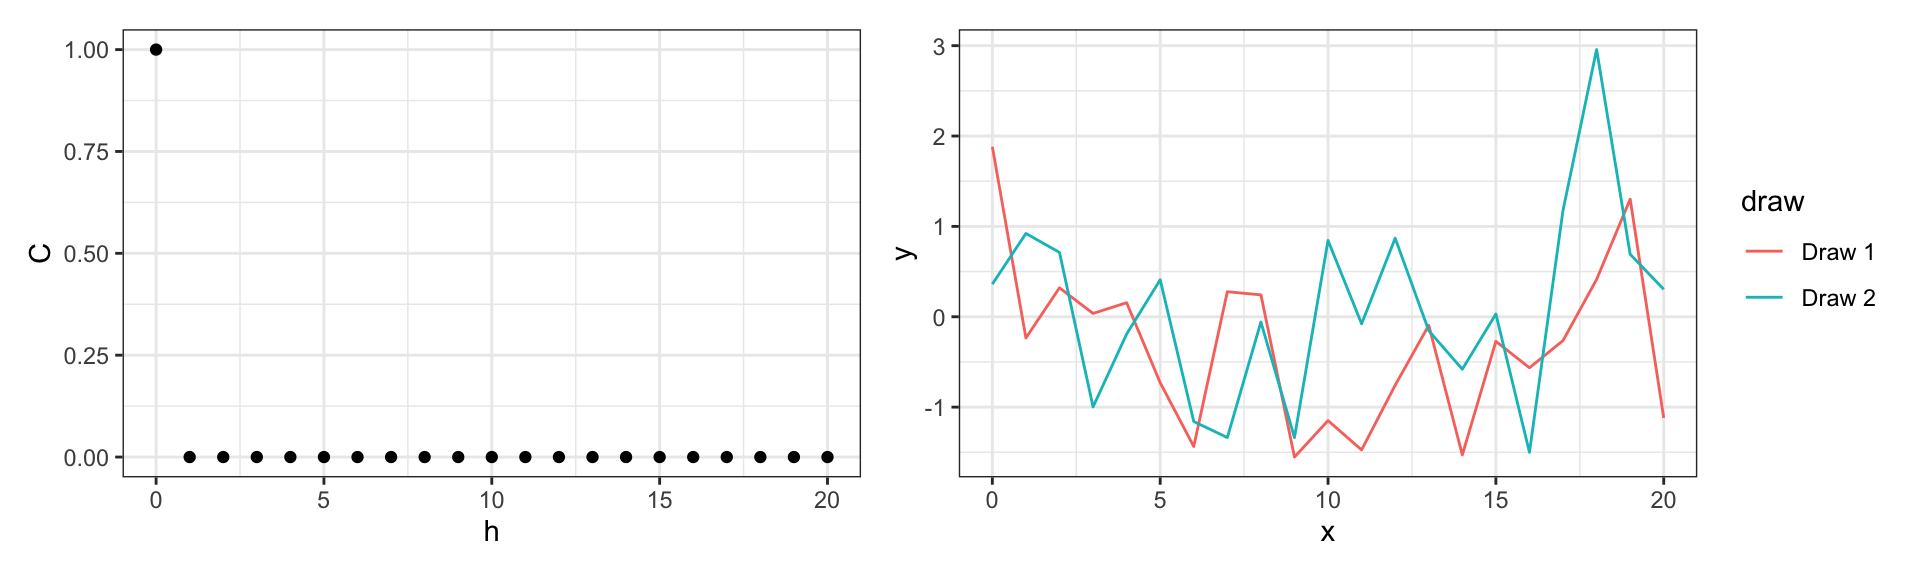
\includegraphics[width=\textwidth]{Lec17_files/figure-beamer/unnamed-chunk-1-1} \end{center}

\end{frame}

\begin{frame}[t]{EDA - Moran's I}
\protect\hypertarget{eda---morans-i}{}

If we have observations at \(n\) spatial locations \((s_1, \ldots s_n)\)

\[ I = \frac{n}{\sum_{i=1}^n \sum_{j=1}^n w_{ij}} \frac{\sum_{i=1}^n \sum_{j=1}^n w_{ij} \big(y(s_i)-\bar{y}\big)\big(y(s_j)-\bar{y}\big)}{\sum_{i=1}^n \big(y(s_i) - \bar{y}\big)^2} \]
where \(\symbf{w} = \{w\}_{ij}\) is a spatial weights matrix.

\pause

\vspace{3mm}

Some properties of Moran's I when there is no spatial autocorrelation /
dependence:

\begin{itemize}
\tightlist
\item
  \(E(I) = -1 / (n-1)\)
\end{itemize}

\vspace{2mm}

\begin{itemize}
\tightlist
\item
  \(Var(I) = \text{Something ugly but closed form}- E(I)^2\)
\end{itemize}

\vspace{2mm}

\begin{itemize}
\tightlist
\item
  \(\underset{n\to\infty}{\lim} \frac{I - E(I)}{\sqrt{Var(I)}} \sim \mathcal{N}(0,1)\)
\end{itemize}

\end{frame}

\begin{frame}[fragile,t]{Adjacency Matrix}
\protect\hypertarget{adjacency-matrix}{}

\scriptoutput

\begin{Shaded}
\begin{Highlighting}[]
\DecValTok{1}\OperatorTok{*}\KeywordTok{st_touches}\NormalTok{(nc[}\DecValTok{1}\OperatorTok{:}\DecValTok{12}\NormalTok{,], }\DataTypeTok{sparse=}\OtherTok{FALSE}\NormalTok{)}
\CommentTok{##       [,1] [,2] [,3] [,4] [,5] [,6] [,7] [,8] [,9] [,10] [,11] [,12]}
\CommentTok{##  [1,]    0    1    0    0    0    0    0    0    0     0     0     0}
\CommentTok{##  [2,]    1    0    1    0    0    0    0    0    0     0     0     0}
\CommentTok{##  [3,]    0    1    0    0    0    0    0    0    0     1     0     0}
\CommentTok{##  [4,]    0    0    0    0    0    0    1    0    0     0     0     0}
\CommentTok{##  [5,]    0    0    0    0    0    1    0    0    1     0     0     0}
\CommentTok{##  [6,]    0    0    0    0    1    0    0    1    0     0     0     0}
\CommentTok{##  [7,]    0    0    0    1    0    0    0    1    0     0     0     0}
\CommentTok{##  [8,]    0    0    0    0    0    1    1    0    0     0     0     0}
\CommentTok{##  [9,]    0    0    0    0    1    0    0    0    0     0     0     0}
\CommentTok{## [10,]    0    0    1    0    0    0    0    0    0     0     0     1}
\CommentTok{## [11,]    0    0    0    0    0    0    0    0    0     0     0     1}
\CommentTok{## [12,]    0    0    0    0    0    0    0    0    0     1     1     0}
\end{Highlighting}
\end{Shaded}

\end{frame}

\begin{frame}[fragile,t]{Normalized Adjacency Matrix}
\protect\hypertarget{normalized-adjacency-matrix}{}

\scriptoutput

\begin{Shaded}
\begin{Highlighting}[]
\NormalTok{normalize_weights =}\StringTok{ }\ControlFlowTok{function}\NormalTok{(w) \{}
  \KeywordTok{diag}\NormalTok{(w) =}\StringTok{ }\DecValTok{0}
\NormalTok{  rs =}\StringTok{ }\KeywordTok{rowSums}\NormalTok{(w)}
\NormalTok{  rs[rs }\OperatorTok{==}\StringTok{ }\DecValTok{0}\NormalTok{] =}\StringTok{ }\DecValTok{1}
\NormalTok{  w}\OperatorTok{/}\NormalTok{rs}
\NormalTok{\}}

\KeywordTok{normalize_weights}\NormalTok{( }\DecValTok{1}\OperatorTok{*}\KeywordTok{st_touches}\NormalTok{(nc[}\DecValTok{1}\OperatorTok{:}\DecValTok{12}\NormalTok{,], }\DataTypeTok{sparse=}\OtherTok{FALSE}\NormalTok{) )}
\CommentTok{##       [,1] [,2] [,3] [,4] [,5] [,6] [,7] [,8] [,9] [,10] [,11] [,12]}
\CommentTok{##  [1,]  0.0  1.0  0.0  0.0  0.0  0.0  0.0  0.0  0.0   0.0   0.0   0.0}
\CommentTok{##  [2,]  0.5  0.0  0.5  0.0  0.0  0.0  0.0  0.0  0.0   0.0   0.0   0.0}
\CommentTok{##  [3,]  0.0  0.5  0.0  0.0  0.0  0.0  0.0  0.0  0.0   0.5   0.0   0.0}
\CommentTok{##  [4,]  0.0  0.0  0.0  0.0  0.0  0.0  1.0  0.0  0.0   0.0   0.0   0.0}
\CommentTok{##  [5,]  0.0  0.0  0.0  0.0  0.0  0.5  0.0  0.0  0.5   0.0   0.0   0.0}
\CommentTok{##  [6,]  0.0  0.0  0.0  0.0  0.5  0.0  0.0  0.5  0.0   0.0   0.0   0.0}
\CommentTok{##  [7,]  0.0  0.0  0.0  0.5  0.0  0.0  0.0  0.5  0.0   0.0   0.0   0.0}
\CommentTok{##  [8,]  0.0  0.0  0.0  0.0  0.0  0.5  0.5  0.0  0.0   0.0   0.0   0.0}
\CommentTok{##  [9,]  0.0  0.0  0.0  0.0  1.0  0.0  0.0  0.0  0.0   0.0   0.0   0.0}
\CommentTok{## [10,]  0.0  0.0  0.5  0.0  0.0  0.0  0.0  0.0  0.0   0.0   0.0   0.5}
\CommentTok{## [11,]  0.0  0.0  0.0  0.0  0.0  0.0  0.0  0.0  0.0   0.0   0.0   1.0}
\CommentTok{## [12,]  0.0  0.0  0.0  0.0  0.0  0.0  0.0  0.0  0.0   0.5   0.5   0.0}
\end{Highlighting}
\end{Shaded}

\end{frame}

\begin{frame}[fragile]{NC SIDS \& Moran's I}
\protect\hypertarget{nc-sids-morans-i}{}

Lets start by using a normalized adjacency matrix for \(\symbf{w}\)
(shared county borders).

\scriptoutput

\begin{Shaded}
\begin{Highlighting}[]
\NormalTok{morans_I =}\StringTok{ }\ControlFlowTok{function}\NormalTok{(y, w) \{}
\NormalTok{  w =}\StringTok{ }\KeywordTok{normalize_weights}\NormalTok{(w)}
\NormalTok{  n =}\StringTok{ }\KeywordTok{length}\NormalTok{(y)}
\NormalTok{  y_bar =}\StringTok{ }\KeywordTok{mean}\NormalTok{(y)}
\NormalTok{  num =}\StringTok{ }\KeywordTok{sum}\NormalTok{(w }\OperatorTok{*}\StringTok{ }\NormalTok{(y}\OperatorTok{-}\NormalTok{y_bar) }\OperatorTok\StringTok{ }\KeywordTok{t}\NormalTok{(y}\OperatorTok{-}\NormalTok{y_bar))  }
\NormalTok{  denom =}\StringTok{ }\KeywordTok{sum}\NormalTok{( (y}\OperatorTok{-}\NormalTok{y_bar)}\OperatorTok{^}\DecValTok{2}\NormalTok{ )}
\NormalTok{  (n}\OperatorTok{/}\KeywordTok{sum}\NormalTok{(w)) }\OperatorTok{*}\StringTok{ }\NormalTok{(num}\OperatorTok{/}\NormalTok{denom)}
\NormalTok{\}}

\NormalTok{w =}\StringTok{ }\DecValTok{1}\OperatorTok{*}\KeywordTok{st_touches}\NormalTok{(nc, }\DataTypeTok{sparse=}\OtherTok{FALSE}\NormalTok{)}

\KeywordTok{morans_I}\NormalTok{(}\DataTypeTok{y =}\NormalTok{ nc}\OperatorTok{$}\NormalTok{SID74, w)}
\CommentTok{## [1] 0.1477405}

\NormalTok{ape}\OperatorTok{::}\KeywordTok{Moran.I}\NormalTok{(nc}\OperatorTok{$}\NormalTok{SID74, }\DataTypeTok{weight =}\NormalTok{ w) }\OperatorTok\StringTok{ }\KeywordTok{str}\NormalTok{()}
\CommentTok{## List of 4}
\CommentTok{##  $ observed: num 0.148}
\CommentTok{##  $ expected: num -0.0101}
\CommentTok{##  $ sd      : num 0.0627}
\CommentTok{##  $ p.value : num 0.0118}
\end{Highlighting}
\end{Shaded}

\end{frame}

\begin{frame}[t]{EDA - Geary's C}
\protect\hypertarget{eda---gearys-c}{}

Like Moran's I, if we have observations at \(n\) spatial locations
\((s_1, \ldots s_n)\)

\[ C = \frac{n-1}{2\sum_{i=1}^n \sum_{j=1}^n w_{ij}} \frac{\sum_{i=1}^n \sum_{j=1}^n w_{ij} \big(y(s_i)-y(s_j)\big)^2}{\sum_{i=1}^n \big(y(s_i) - \bar{y}\big)^2} \]
where \(\symbf{w}\) is a spatial weights matrix.

\pause

\vspace{7mm}

Some properties of Geary's C:

\begin{itemize}
\tightlist
\item
  \(0 < C < 2\)

  \begin{itemize}
  \tightlist
  \item
    If \(C \approx 1\) then no spatial autocorrelation
  \item
    If \(C > 1\) then negative spatial autocorrelation
  \item
    If \(C < 1\) then positive spatial autocorrelation
  \end{itemize}
\item
  Geary's C is inversely related to Moran's I
\end{itemize}

\end{frame}

\begin{frame}[fragile,t]{NC SIDS \& Geary's C}
\protect\hypertarget{nc-sids-gearys-c}{}

Again using an normalized adjacency matrix for \(\symbf{w}\) (shared
county borders).

\scriptoutput

\begin{Shaded}
\begin{Highlighting}[]
\NormalTok{gearys_C =}\StringTok{ }\ControlFlowTok{function}\NormalTok{(y, w) \{}
\NormalTok{  w =}\StringTok{ }\KeywordTok{normalize_weights}\NormalTok{(w)}
  
\NormalTok{  n =}\StringTok{ }\KeywordTok{length}\NormalTok{(y)}
\NormalTok{  y_bar =}\StringTok{ }\KeywordTok{mean}\NormalTok{(y)}
\NormalTok{  y_i =}\StringTok{ }\NormalTok{y }\OperatorTok\StringTok{ }\KeywordTok{t}\NormalTok{(}\KeywordTok{rep}\NormalTok{(}\DecValTok{1}\NormalTok{,n))}
\NormalTok{  y_j =}\StringTok{ }\KeywordTok{t}\NormalTok{(y_i)}
\NormalTok{  num =}\StringTok{ }\KeywordTok{sum}\NormalTok{(w }\OperatorTok{*}\StringTok{ }\NormalTok{(y_i}\OperatorTok{-}\NormalTok{y_j)}\OperatorTok{^}\DecValTok{2}\NormalTok{)  }
\NormalTok{  denom =}\StringTok{ }\KeywordTok{sum}\NormalTok{( (y}\OperatorTok{-}\NormalTok{y_bar)}\OperatorTok{^}\DecValTok{2}\NormalTok{ )}
\NormalTok{  ((n}\DecValTok{-1}\NormalTok{)}\OperatorTok{/}\NormalTok{(}\DecValTok{2}\OperatorTok{*}\KeywordTok{sum}\NormalTok{(w))) }\OperatorTok{*}\StringTok{ }\NormalTok{(num}\OperatorTok{/}\NormalTok{denom)}
\NormalTok{\}}

\NormalTok{w =}\StringTok{ }\DecValTok{1}\OperatorTok{*}\KeywordTok{st_touches}\NormalTok{(nc, }\DataTypeTok{sparse=}\OtherTok{FALSE}\NormalTok{)}

\KeywordTok{gearys_C}\NormalTok{(}\DataTypeTok{y =}\NormalTok{ nc}\OperatorTok{$}\NormalTok{SID74, }\DataTypeTok{w =}\NormalTok{ w)}
\CommentTok{## [1] 0.8438767}
\end{Highlighting}
\end{Shaded}

\end{frame}

\begin{frame}[fragile]{Spatial Correlogram}
\protect\hypertarget{spatial-correlogram}{}

\scriptoutput

\begin{Shaded}
\begin{Highlighting}[]
\NormalTok{nc_pt =}\StringTok{ }\KeywordTok{st_centroid}\NormalTok{(nc)}
\KeywordTok{plot}\NormalTok{(nc_pt[,}\StringTok{"SID74"}\NormalTok{], }\DataTypeTok{pch=}\DecValTok{16}\NormalTok{)}
\end{Highlighting}
\end{Shaded}

\begin{center}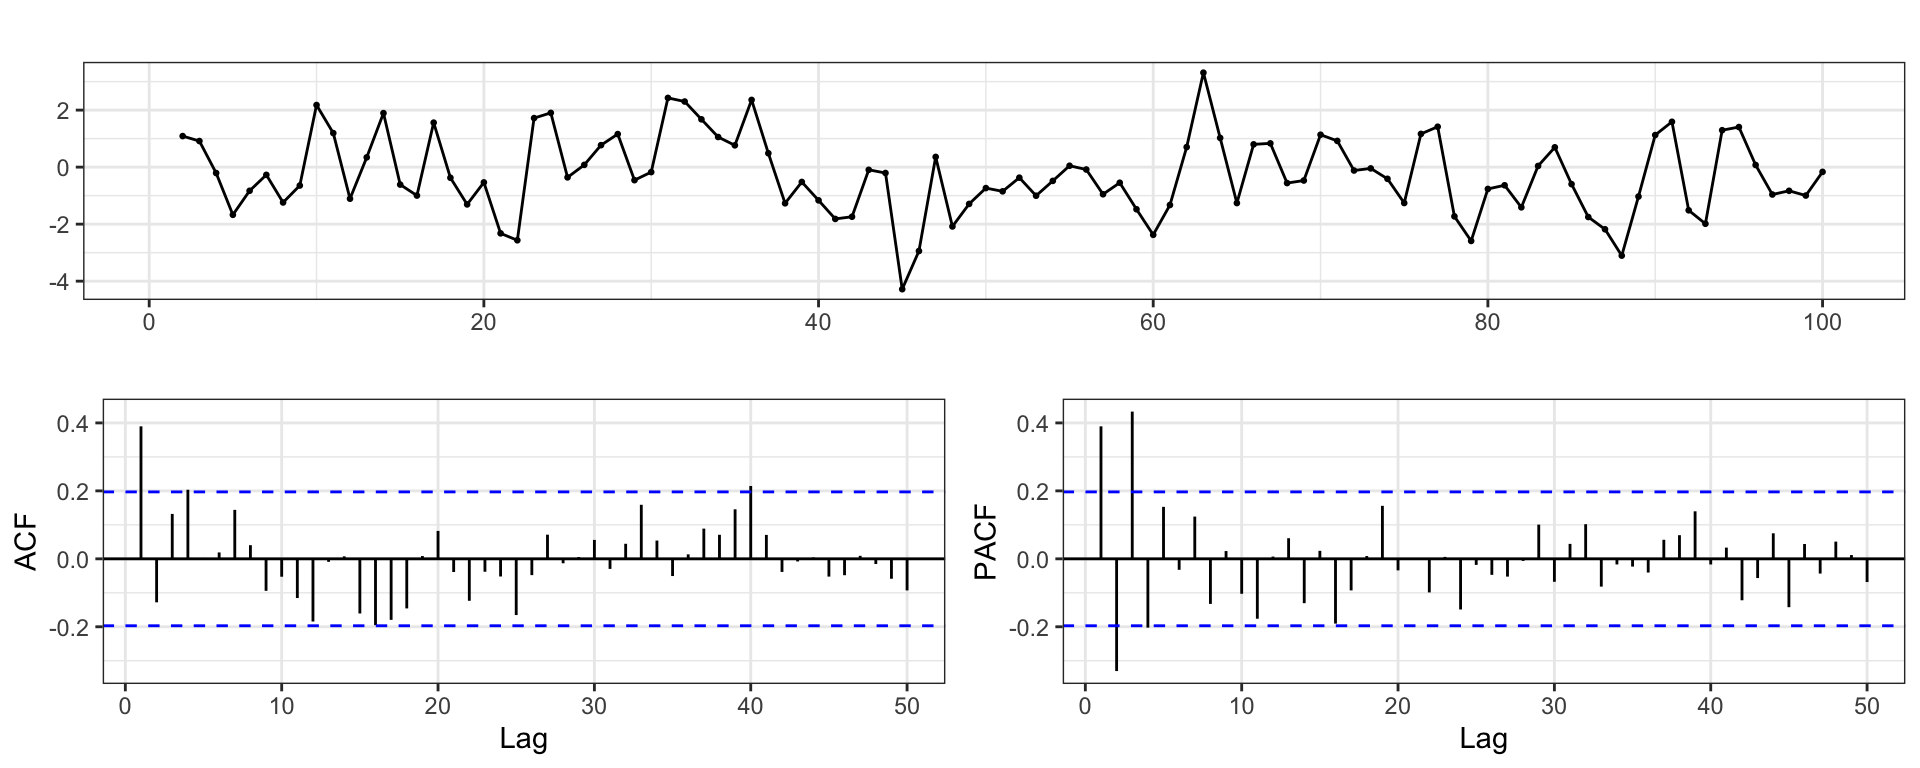
\includegraphics[width=\textwidth,height=0.5\textheight]{Lec17_files/figure-beamer/unnamed-chunk-6-1} \end{center}

\end{frame}

\begin{frame}{}
\protect\hypertarget{section}{}

\begin{center}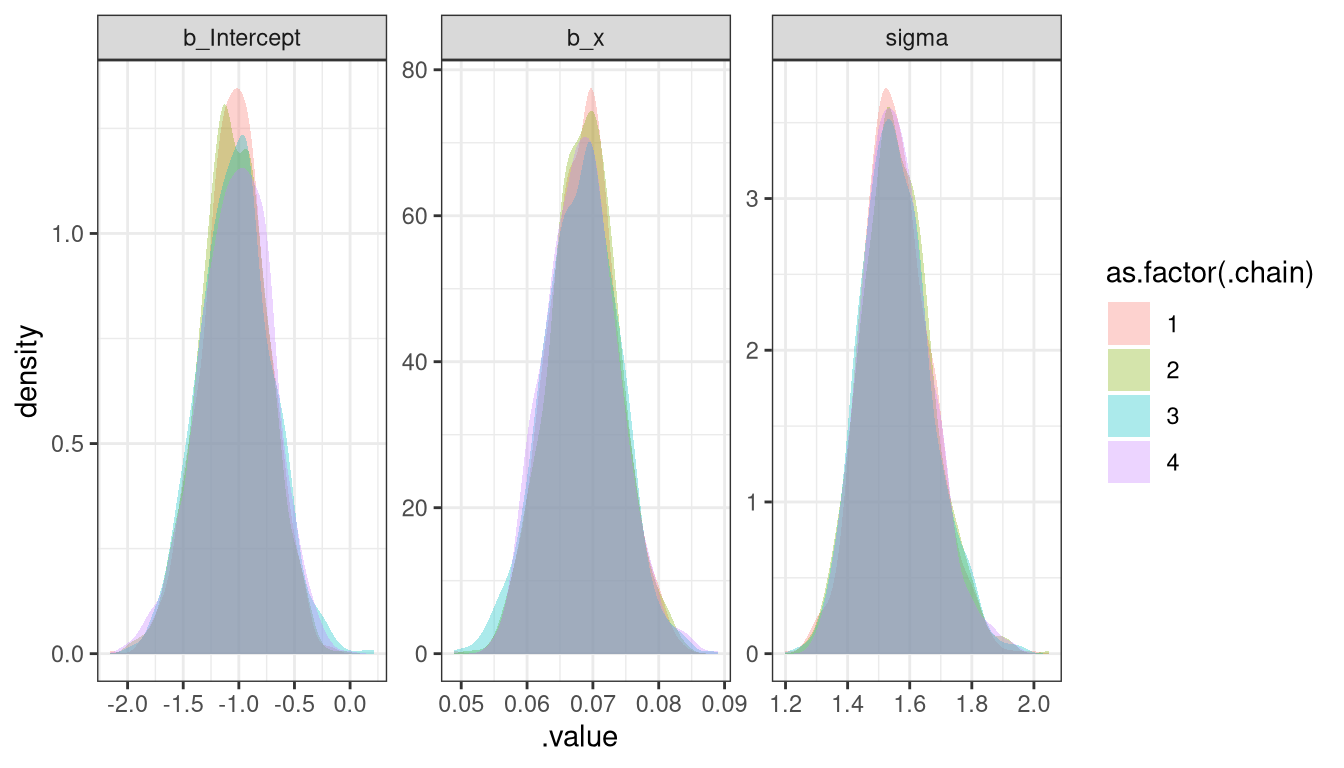
\includegraphics[width=\textwidth]{Lec17_files/figure-beamer/unnamed-chunk-7-1} \end{center}

\end{frame}

\begin{frame}{}
\protect\hypertarget{section-1}{}

\begin{center}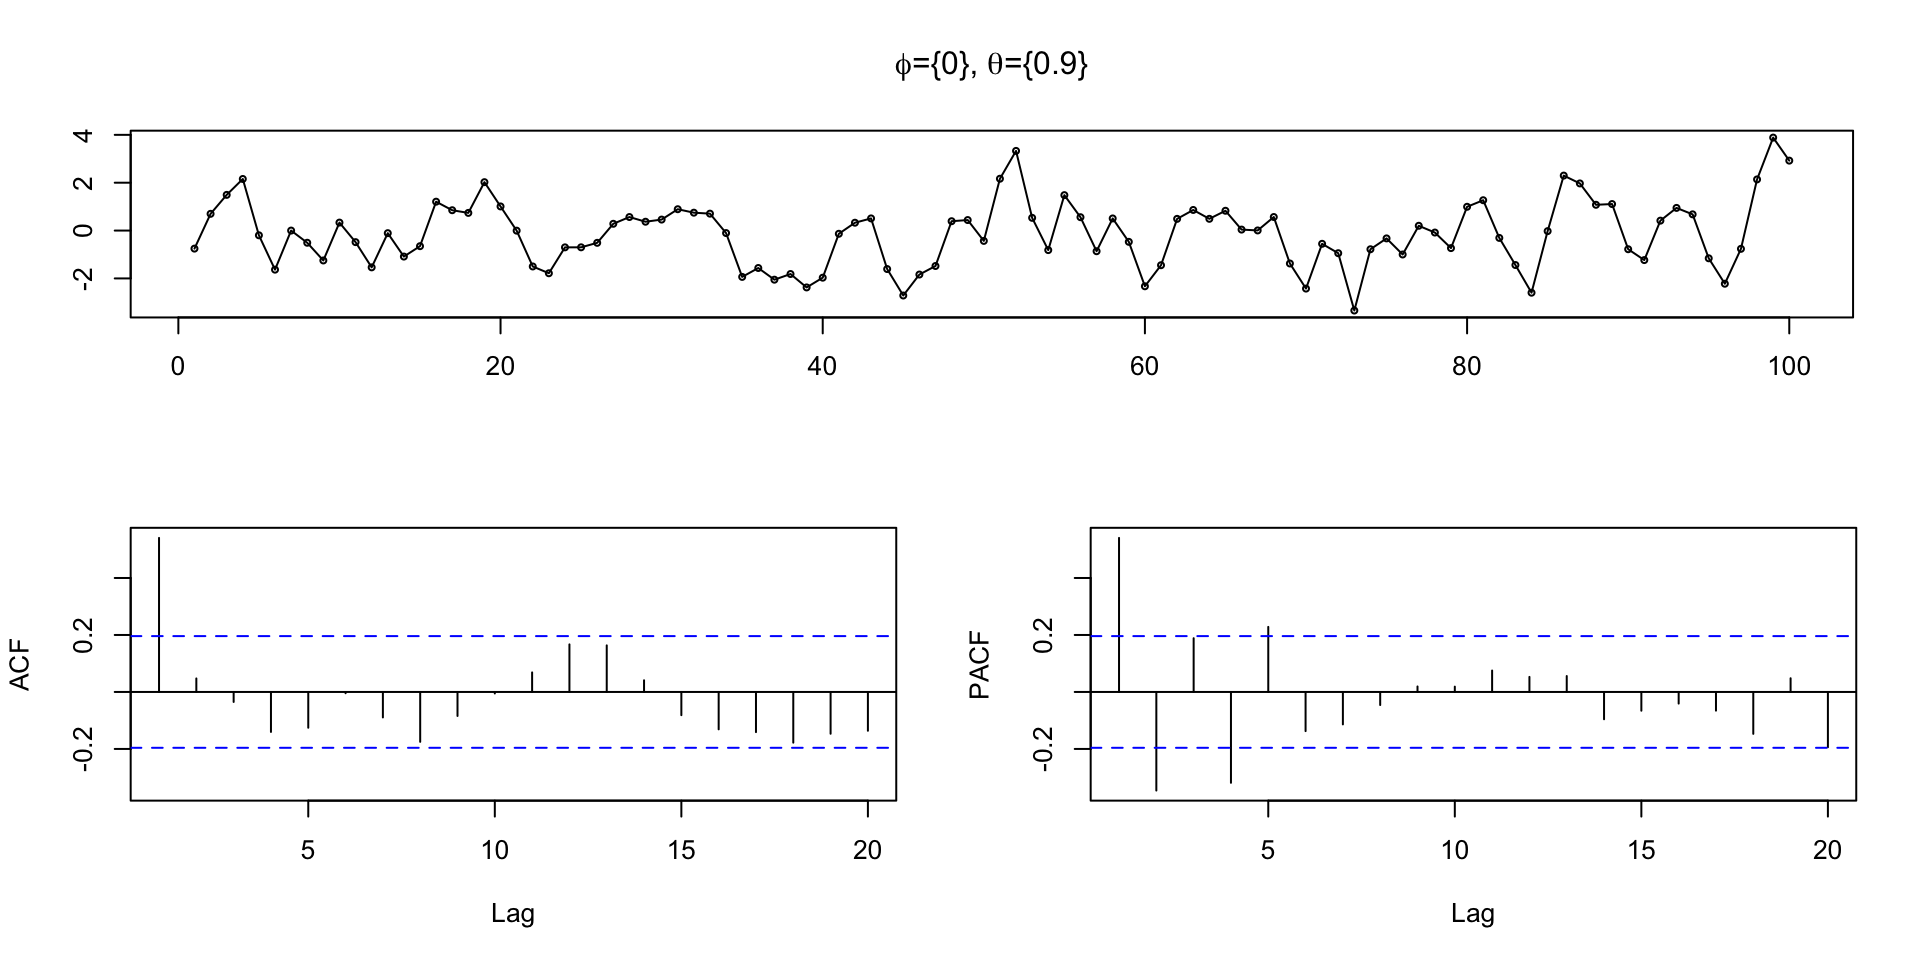
\includegraphics[width=\textwidth]{Lec17_files/figure-beamer/unnamed-chunk-8-1} \end{center}

\end{frame}

\hypertarget{autoregressive-models}{%
\section{Autoregressive Models}\label{autoregressive-models}}

\begin{frame}[t]{AR Models - Time}
\protect\hypertarget{ar-models---time}{}

Lets just focus on the simplest case, an \(AR(1)\) process

\[ y_t = \delta + \phi \, y_{t-1} + w_t \]

where \(w_t \sim \mathcal{N}(0,\sigma^2)\) and \(|\phi| < 1\), then

\[
\begin{aligned}
E(y_t) &= \frac{\delta}{1-\phi} \\
Var(y_t) &= \frac{\sigma^2}{1-\phi} \\
\rho(h) &= \phi^{h} \\
\gamma(h) &=  \phi^h \frac{\sigma^2}{1-\phi}
\end{aligned}
\]

\end{frame}

\begin{frame}[t]{AR Models - Time - Joint Distribution}
\protect\hypertarget{ar-models---time---joint-distribution}{}

Previously we saw that an \(AR(1)\) model can be represented using a
multivariate normal distribution

\[
\begin{pmatrix}
y_1 \\ y_2 \\ \vdots \\ y_n
\end{pmatrix}
\sim \mathcal{N} \begin{pmatrix}
\frac{\delta}{1-\phi} \begin{pmatrix}1\\ 1\\ \vdots\\ 1\end{pmatrix},~
\frac{\sigma^2}{1-\phi}
\begin{pmatrix}
1      & \phi   & \cdots & \phi^{n-1} \\
\phi   & 1      & \cdots & \phi^{n-2} \\
\vdots & \vdots & \ddots & \vdots     \\
\phi^{n-1} & \phi^{n-2}  & \cdots & 1 \\
\end{pmatrix}
\end{pmatrix}
\]

\pause

\vspace{2mm}

In writing down the likelihood we also saw that an \(AR(1)\) is 1st
order Markovian,

\[ \begin{aligned}
f(y_1, \ldots, y_n) 
  &= f(y_1) \, f(y_2 | y_1) \,  f(y_3|y_2,y_1) \,\cdots\, f(y_n|y_{n-1},y_{n-2},\ldots,y_1) \\
  &= f(y_1) \, f(y_2 | y_1) \,  f(y_3|y_2) \,\cdots\, f(y_n|y_{n-1})
\end{aligned} \]

\end{frame}

\begin{frame}{Alternative Definitions for \(y_t\)}
\protect\hypertarget{alternative-definitions-for-y_t}{}

\Large

\[ y_t = \delta + \phi \, y_{t-1} + w_t \]

\vspace{2mm}

\begin{center}vs.\end{center}

\vspace{2mm}

\[ y_t | y_{t-1} \sim \mathcal{N}(\delta + \phi \, y_{t-1},~\sigma^2) \]

\pause

\vspace{3mm}
\normalsize

In the case of time, both of these definitions result in the same
multivariate distribution for \(\symbf{y}\).

\end{frame}

\begin{frame}[t]{AR in Space}
\protect\hypertarget{ar-in-space}{}

\vspace{4mm}

\begin{center}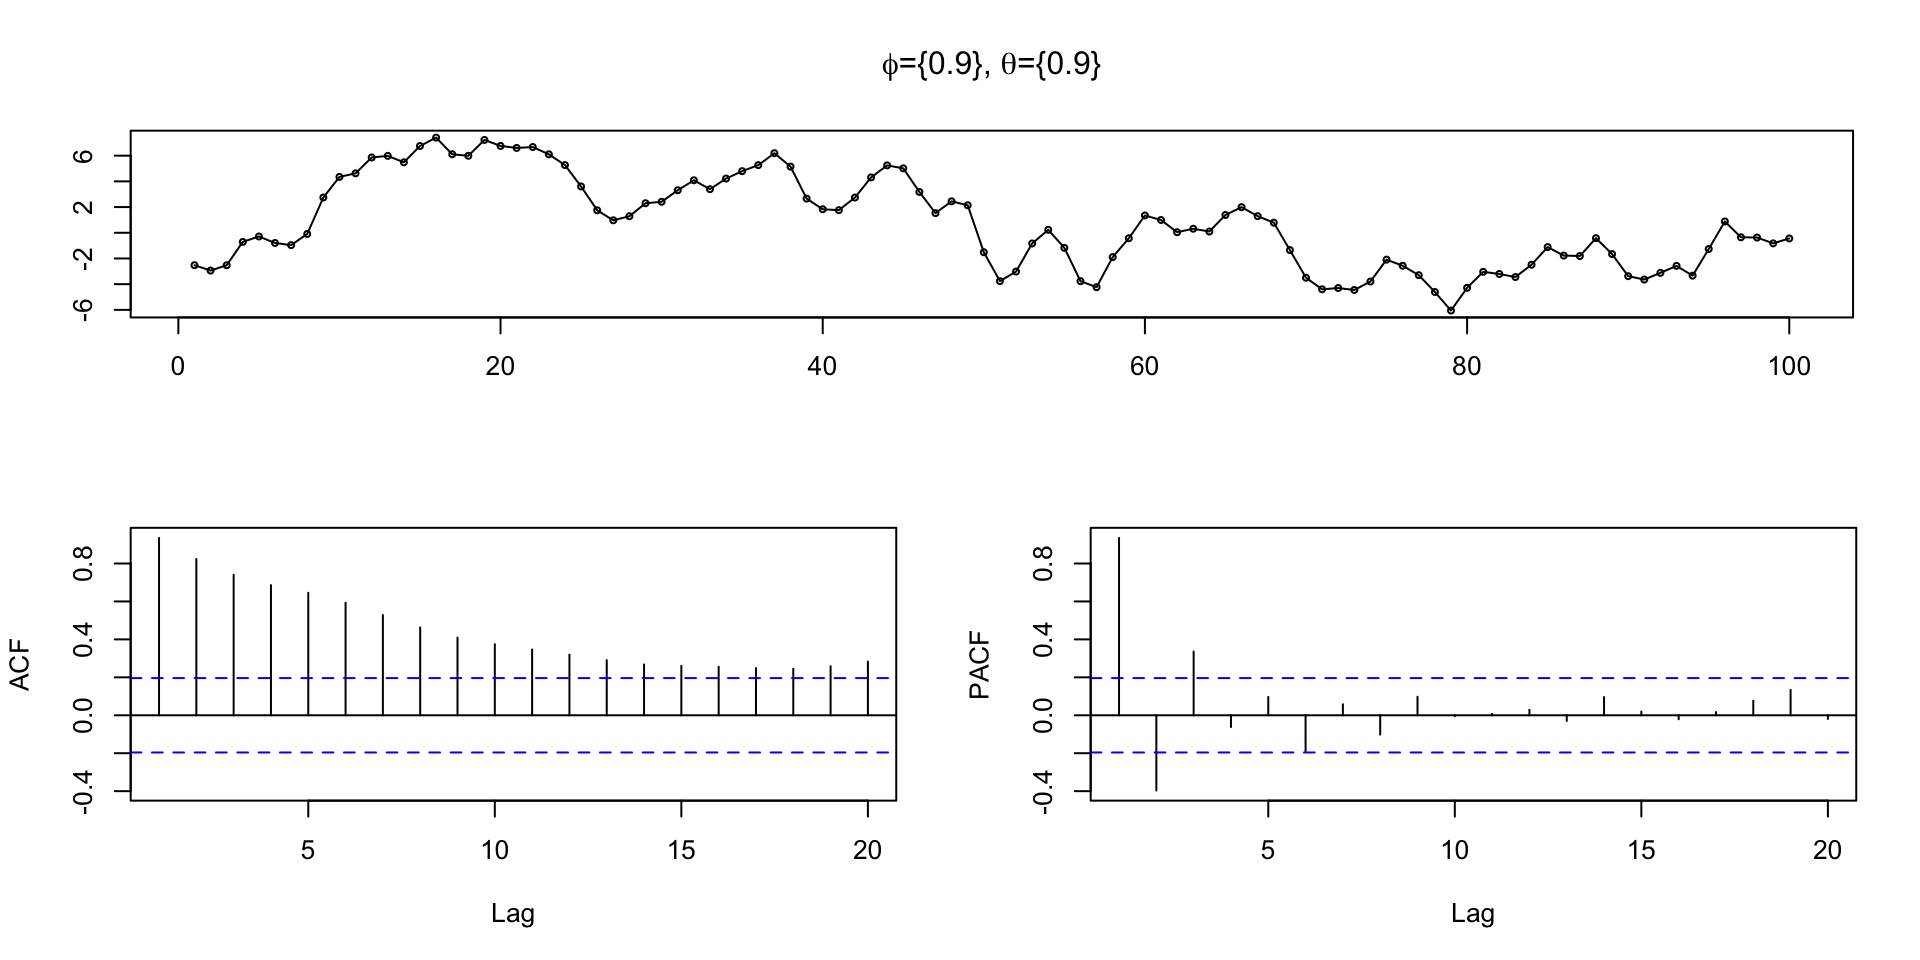
\includegraphics[width=\textwidth]{Lec17_files/figure-beamer/unnamed-chunk-9-1} \end{center}

\pause

Even in the simplest spatial case there is no clear / unique ordering,
\scriptsize \[ \begin{aligned}
f\big(y(s_1), \ldots, y(s_{10})\big) 
  &= f\big(y(s_1)\big) \, f\big(y(s_2) | y(s_1)\big) \, \cdots \, f\big(y(s_{10} | y(s_{9}),y(s_{8}),\ldots,y(s_1)\big)  \\
  &= f\big(y(s_{10})\big) \, f\big(y(s_9) | y(s_{10})\big) \, \cdots \, f\big(y(s_{1} | y(s_{2}),y(s_{3}),\ldots,y(s_{10})\big)  \\
  &= ~?
\end{aligned} \] \normalsize

\pause

Instead we need to think about things in terms of their neighbors /
neighborhoods. We define \(N(s_i)\) to be the set of neighbors of
location \(s_i\).

\begin{itemize}
\item
  If we define the neighborhood based on ``touching'' then
  \(N(s_3) = \{s_2, s_4\}\)
\item
  If we use distance within 2 units then
  \(N(s_3) = \{s_1,s_2,s_3,s_4\}\)
\end{itemize}

\end{frame}

\begin{frame}[t]{Defining the Spatial AR model}
\protect\hypertarget{defining-the-spatial-ar-model}{}

Here we will consider a simple average of neighboring observations, just
like with the temporal AR model we have two options in terms of defining
the autoregressive process,

\pause

\begin{itemize}
\tightlist
\item
  Simultaneous Autogressve (SAR)
\end{itemize}

\[ y(s) = \delta + \phi \frac{1}{|N(s)|}\sum_{s' \in N(s)} y(s') + \mathcal{N}(0,\sigma^2) \]

\pause

\begin{itemize}
\tightlist
\item
  Conditional Autoregressive (CAR)
\end{itemize}

\[ y(s)|\symbf{y}(-s) \sim \mathcal{N}\left(\delta + \phi \frac{1}{|N(s)|}\sum_{s' \in N(s)} y(s'),~ \sigma^2 \right) \]

\end{frame}

\begin{frame}[t]{Simultaneous Autogressve (SAR)}
\protect\hypertarget{simultaneous-autogressve-sar}{}

\vspace{-3mm}

Using
\[ y(s) = \phi \frac{1}{|N(s)|}\sum_{s' \in N(s)} y(s') + \mathcal{N}(0,\sigma^2) \]
we want to find the distribution of
\(\symbf{y} = \Big(y(s_1),\, y(s_2),\,\ldots,\,y(s_n)\Big)^t\).

\pause

\vspace{5mm}

First we can define a weight matrix \(\symbf{W}\) where \[ 
\{\symbf{W}\}_{ij} = \begin{cases}
1/|N(s_i)| & \text{if $j \in N(s_i)$} \\
0        & \text{otherwise}
\end{cases}
\] then we can write \(\symbf{y}\) as follows,
\[ \symbf{y} = \phi \, \symbf{W} \, \symbf{y} + \symbf{\epsilon} \]
where \[ \symbf{\epsilon} \sim \mathcal{N}(0,\sigma^2 \, \symbf{I}) \]

\end{frame}

\begin{frame}[t]{A toy example}
\protect\hypertarget{a-toy-example}{}

\begin{center}
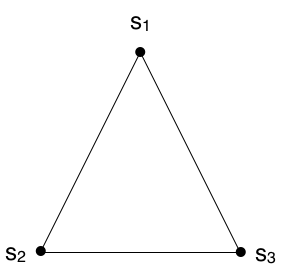
\includegraphics[width=0.3\textwidth]{figs/triangle_adj.png} \\
\end{center}

\end{frame}

\begin{frame}[t]{Back to SAR}
\protect\hypertarget{back-to-sar}{}

\[ \symbf{y} = \phi \, \symbf{W} \, \symbf{y} + \symbf{\epsilon} \]

\end{frame}

\begin{frame}[t]{Conditional Autogressve (CAR)}
\protect\hypertarget{conditional-autogressve-car}{}

This is a bit trickier, in the case of the temporal AR process we
actually went from joint distribution \(\to\) conditional distributions
(which we were then able to simplify).

\vspace{3mm}

Since we don't have a natural ordering we can't get away with this (at
least not easily).

\vspace{3mm}

Going the other way, conditional distributions \(\to\) joint
distribution is difficult because it is possible to specify conditional
distributions that lead to an improper joint distribution.

\end{frame}

\begin{frame}[t]{Brooks' Lemma}
\protect\hypertarget{brooks-lemma}{}

For sets of observations \(\symbf{x}\) and \(\symbf{y}\) where
\(p(x) > 0~~\forall ~ x\in\symbf{x}\) and
\(p(y) > 0~~\forall ~ y\in\symbf{y}\) then

\[\begin{aligned}
\frac{p(\symbf{y})}{p(\symbf{x})} 
  &= \prod_{i=1}^n \frac{p(y_i ~|~ y_1,\ldots,y_{i-1},x_{i+1},\ldots,x_n)}{p(x_i ~|~ y_1,\ldots,y_{i-1},x_{i+1},\ldots,x_n)} \\
  &= \prod_{i=1}^n \frac{p(y_i ~|~ x_1,\ldots,x_{i-1},y_{i+1},\ldots,y_n)}{p(x_i ~|~ x_1,\ldots,x_{i-1},y_{i+1},\ldots,y_n)} \\
\end{aligned}\]

\end{frame}

\begin{frame}{A simplified example}
\protect\hypertarget{a-simplified-example}{}

Let \(\symbf{y} = (y_1,y_2)\) and \(\symbf{x} = (x_1,x_2)\) then we can
derive Brook's Lemma for this case,

\begin{align*}
\action<+->{
  p (y_1,y_2) 
    &= p(y_1 | y_2) p(y_2) \\
}
\action<+->{
    &= p(y_1 | y_2) \frac{p(y_2|x_1)}{p(x_1|y_2)} p(x_1)
}
\action<+->{
    = \frac{p(y_1 | y_2)}{p(x_1 | y_2)} p(y_2|x_1) \, p(x_1) \\
}
\action<+->{
    & = \frac{p(y_1 | y_2)}{p(x_1 | y_2)} p(y_2|x_1) \, p(x_1)   \left(\frac{p(x_2|x_1)}{p(x_2|x_1)}\right) \\
}
\action<+->{
    & = \frac{p(y_1 | y_2)}{p(x_1 | y_2)} \frac{p(y_2|x_1)}{p(x_2|x_1)} \, p(x_1,x_2) \\
  \\
}
\action<+->{
  \frac{p (y_1,y_2) }{p(x_1,x_2)} 
    & = \frac{p(y_1 | y_2)}{p(x_1 | y_2)} \frac{p(y_2|x_1)}{p(x_2|x_1)}
}
\end{align*}

\end{frame}

\begin{frame}[t]{Utility?}
\protect\hypertarget{utility}{}

Lets repeat that last example but consider the case where
\(\symbf{y} = (y_1,y_2)\) but now we let \(\symbf{x} = (y_1=0,y_2=0)\)

\begin{align*}
\action<+->{
  \frac{p (y_1,y_2) }{p(x_1,x_2)} 
    &= \frac{p (y_1,y_2) }{p(y_1=0,y_2=0)}  \\
  \\
}
\action<+->{
  p(y_1,y_2) &= \frac{p(y_1 | y_2)}{p(y_1=0 | y_2)} \frac{p(y_2|y_1=0)}{p(y_2=0|y_1=0)} ~ p(y_1=0,y_2=0) \\
  \\
}
\action<+->{
  p(y_1,y_2) 
    &\propto \frac{p(y_1 | y_2) ~ p(y_2|y_1=0) }{ p(y_1=0 | y_2)} \\
    &\propto \frac{p(y_2 | y_1) ~ p(y_1|y_2=0) }{ p(y_2=0 | y_1)}
}
\end{align*}

\end{frame}

\begin{frame}[t]{As applied to a \textbf{simple} CAR}
\protect\hypertarget{as-applied-to-a-simple-car}{}

\begin{center}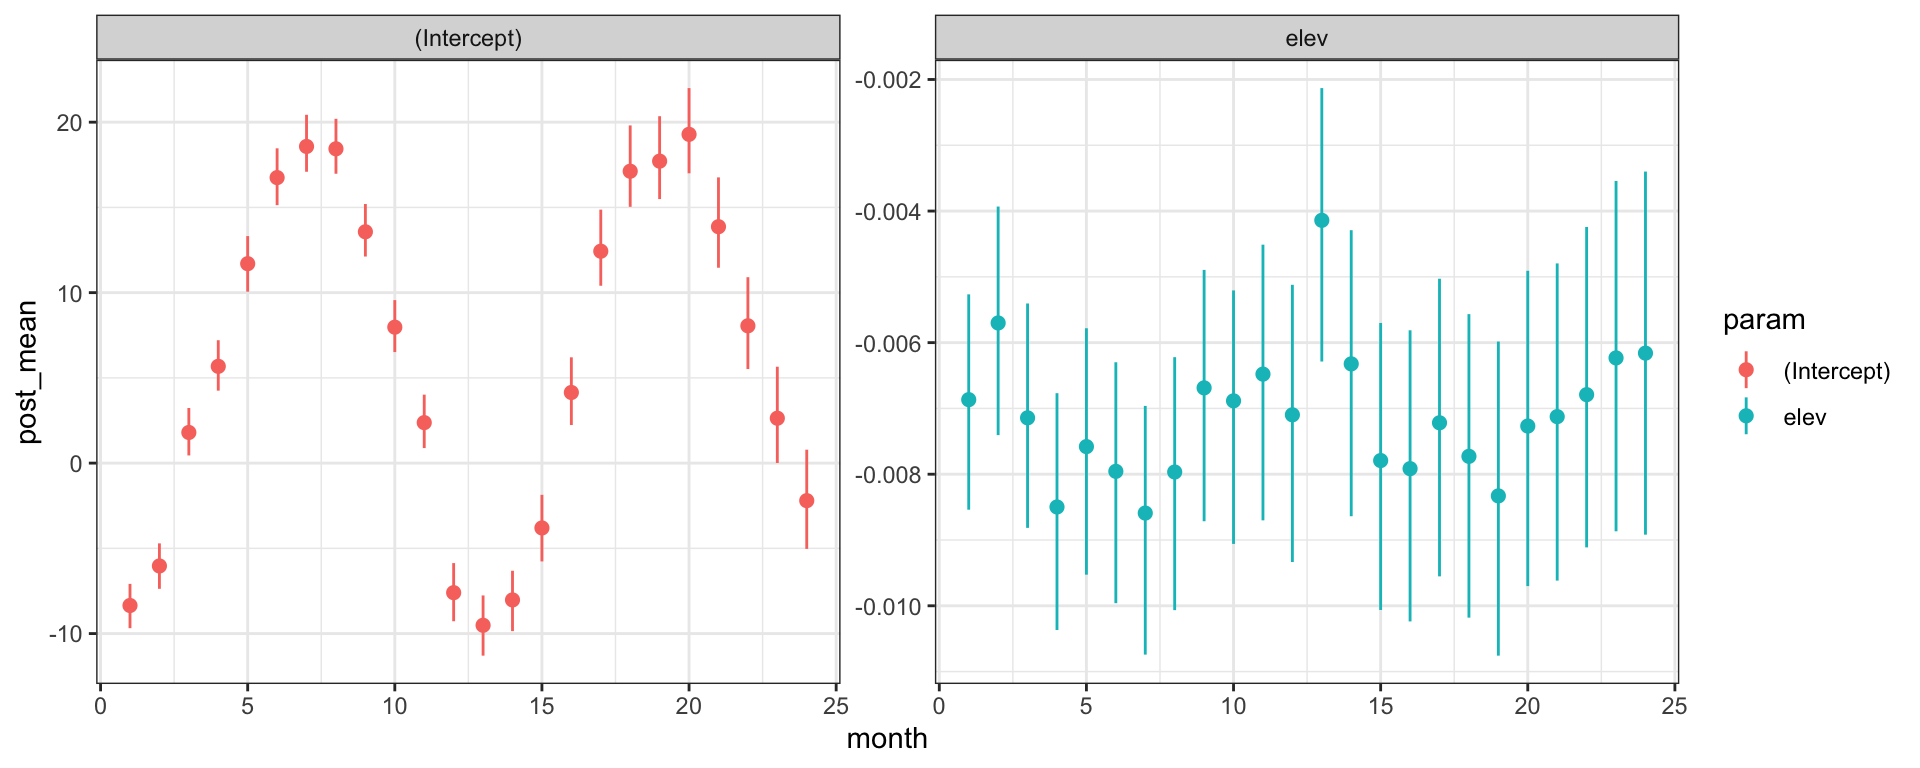
\includegraphics[width=0.2\textwidth]{Lec17_files/figure-beamer/unnamed-chunk-10-1} \end{center}

\scriptsize

\[ \begin{aligned}
y(s_1) | y(s_2) \sim \mathcal{N}(\phi W_{12}\, y(s_2), \sigma^2) \\
y(s_2) | y(s_1) \sim \mathcal{N}(\phi W_{21}\, y(s_1), \sigma^2)
\end{aligned}\]

\pause

\begin{align*}
\action<+->{
  p\big(y(s_1),y(s_2)\big) 
    &\propto \frac{p\big(y(s_1) | y(s_2)\big) ~   p\big(y(s_2)|y(s_1)=0\big)}{p\big(y(s_1)=0|y(s_2)\big)}\\
}
\action<+->{
    &\propto 
      \frac{
        \exp\left(-\frac{1}{2\sigma^2}\left(y(s_1)-\phi \, W_{12} \,   y(s_2)\right)^2\right)
        \exp\left(-\frac{1}{2\sigma^2}\left(y(s_2)-\phi \, W_{21} \, 0\right)^2\right) 
      }{
        \exp\left(-\frac{1}{2\sigma^2}\left(0-\phi W_{12} y(s_2)\right)^2 \right)
      }\\
}
\action<+->{
    &\propto \exp\left(-\frac{1}{2\sigma^2}\left(\left(y(s_1)-\phi \, W_{12} \,   y(s_2)\right)^2 + y(s_2)^2- (\phi W_{21} y(s_2))^2\right)\right) \\
}
\action<+->{
    &\propto \exp\left(-\frac{1}{2\sigma^2}\left(y(s_1)^2-\phi \, W_{12} \,   y(s_1)\,y(s_2) -\phi \, W_{21} \,   y(s_1)\,y(s_2) + y(s_2)^2\right)\right) \\
}
\action<+->{
    &\propto \exp\left(-\frac{1}{2\sigma^2} (\symbf{y}-0)
      \begin{pmatrix} 
      1 & -\phi W_{12} \\
      -\phi W_{21} & 1
      \end{pmatrix}
      (\symbf{y}-0)^{t}
    \right)
}
\end{align*}

\end{frame}

\begin{frame}{Implications for \(\symbf{y}\)}
\protect\hypertarget{implications-for-symbfy}{}

\vspace{-3mm}

\[ \symbf{\mu} = 0 \]

\pause

\[
\begin{aligned}
\symbf{\Sigma}^{-1} &= \frac{1}{\sigma^2}
  \begin{pmatrix} 
    1 & -\phi W_{12} \\
    -\phi W_{21} & 1
  \end{pmatrix} \\
  &= \frac{1}{\sigma^2}(\symbf{I} - \phi \, \symbf{W})
\end{aligned}
\]

\pause

\[
\symbf{\Sigma} = \sigma^2(\symbf{I} - \phi \, \symbf{W})^{-1}
\]

\pause

we can then conclude that for \(\symbf{y} = (y(s_1),~y(s_2))^t\),

\[
\symbf{y} \sim \mathcal{N}\left(
\symbf{0}, ~
\sigma^2 (\symbf{I} - \phi \, \symbf{W})^{-1}
\right)
\]

which generalizes for all mean 0 CAR models.

\end{frame}

\begin{frame}{General Proof}
\protect\hypertarget{general-proof}{}

Let \(\symbf{y} = (y(s_1),\ldots,y(s_n))\) and
\(\symbf{0} = (y(s_1) = 0, \ldots, y(s_n)=0)\) then by Brook's lemma,

\scriptsize

\begin{align*}
\action<+->{
  \frac{p(\symbf{y})}{p(\symbf{0})} 
    &= \prod_{i=1}^n \frac{p(y_i|y_1,\ldots,y_{i-1},0_{i+1},\ldots,0_{n})}{p(0_i|y_1,\ldots,y_{i-1},0_{i+1},\ldots,0_{n})} \\
}
\action<+->{
  &= \prod_{i=1}^n 
    \frac{
      \exp\left(-\frac{1}{2\sigma^2} \left(y_i - \phi \sum_{j<i} W_{ij} \, y_j - \phi \sum_{j>i} 0_j \right)^2 \right)
    }{
      \exp\left(-\frac{1}{2\sigma^2} \left(0_i - \phi \sum_{j<i} W_{ij} \, y_j - \phi \sum_{j>i} 0_j \right)^2 \right)
    } \\
}
\action<+->{
  &= \exp\left(-\frac{1}{2\sigma^2} \sum_{i=1}^n \left(y_i - \phi \sum_{j<i} W_{ij} \, y_j\right)^2 + \frac{1}{2\sigma^2} \sum_{i=1}^n \left( \phi \sum_{j<i} W_{ij} \, y_j \right)^2 \right) \\
}
\action<+->{
  &= \exp\left(-\frac{1}{2\sigma^2} \sum_{i=1}^n y_i^2 - 2 \phi y_i \,\sum_{j<i} W_{ij} \, y_j \right) \\
}
\action<+->{  
  &= \exp\left(-\frac{1}{2\sigma^2} \sum_{i=1}^n y_i^2 - \phi \sum_{i=1}^n \sum_{j=1}^n y_i \, W_{ij} \, y_j \right) \quad \mathit{\big(\text{if } W_{ij} = W_{ji}\big)} \\
}
\action<+->{
  &= \exp\left(-\frac{1}{2\sigma^2} (\symbf{y}-0)^t (\symbf{I} - \phi \symbf{W}) (\symbf{y}-0)  \right)
}
\end{align*}

\end{frame}

\begin{frame}[t]{CAR vs SAR}
\protect\hypertarget{car-vs-sar}{}

\begin{itemize}
\tightlist
\item
  Simultaneous Autogressve (SAR)
\end{itemize}

\[ y(s) = \phi \sum_{s'} W_{s\,s'} \, y(s') + \epsilon \]

\[ \symbf{y} \sim \mathcal{N}(0,~\sigma^2 \, ((\symbf{I}-\phi \symbf{W})^{-1}) ((\symbf{I}-\phi \symbf{W})^{-1})^t )\]

\begin{itemize}
\tightlist
\item
  Conditional Autoregressive (CAR)
\end{itemize}

\[ y(s)|\symbf{y}(-s) \sim \mathcal{N}\left(\sum_{s'} W_{s\,s'} \, y(s'),~ \sigma^2 \right) \]

\[ \symbf{y} \sim \mathcal{N}(0,~\sigma^2 \, (\symbf{I}-\phi \symbf{W})^{-1})\]

\end{frame}

\begin{frame}[t]{Generalization}
\protect\hypertarget{generalization}{}

\begin{itemize}
\item
  Adopting different weight matrices, \(\symbf{W}\)

  \begin{itemize}
  \item
    Between SAR and CAR model we move to a generic weight matrix
    definition (beyond average of nearest neighbors)
  \item
    In time we varied \(p\) in the \(AR(p)\) model, in space we adjust
    the weight matrix.
  \item
    In general having a symmetric W is helpful, but not required
  \end{itemize}
\end{itemize}

\pause

\begin{itemize}
\item
  More complex Variance (beyond \(\sigma^2 \, I\))

  \begin{itemize}
  \item
    \(\sigma^2\) can be a vector (differences between areal locations)
  \item
    i.e.~since areal data tends to be aggregated - adjust variance based
    on sample size
  \item
    i.e.~scale based on the number of neighbors
  \end{itemize}
\end{itemize}

\end{frame}

\begin{frame}[t]{Some specific generalizations}
\protect\hypertarget{some-specific-generalizations}{}

Generally speaking we will want to work with a scaled / normalized
version of the weight matrix,
\[ \frac{W_{ij}}{W_{i\boldsymbol{\cdot}}}  \]

When \(W\) is derived from an adjacency matrix, \(\symbf{A}\), we can
express this as \[ \symbf{W} = \symbf{D}^{-1} \symbf{A} \] where
\(\symbf{D}^{-1} = \text{diag}(1/|N(s_i)|)\).

We can also allow \(\sigma^2\) to vary between locations, we can define
this as \(\symbf{D}_{\sigma^2} = \text{diag}(\sigma^2_i)\) and most
often we use
\[ \symbf{D}_{\sigma^2}^{-1} = \text{diag}\left(\frac{\sigma^2}{|N(s_i)|}\right) =  \sigma^2 \symbf{D}^{-1}.  \]

\end{frame}

\begin{frame}[t]{Revised SAR Model}
\protect\hypertarget{revised-sar-model}{}

\begin{itemize}
\tightlist
\item
  Formula Model
  \[ y(s_i) = X_{i\cdot}\beta + \phi \sum_{j=1}^n D^{-1}_{jj} \, A_{ij} \, \big(y(s_j) - X_{j\cdot}\beta\big) + \epsilon_i \]
  \[ \symbf{\epsilon} \sim \mathcal{N}(\symbf{0},\,\symbf{D}_{\sigma^2}^{-1}) =  \mathcal{N}(\symbf{0},\, \sigma^2 \symbf{D}^{-1}) \]
\item
  Joint Model \pause
  \[\symbf{y} = \symbf{X}\symbf{\beta} + \phi \symbf{D}^{-1} \symbf{A} ~\big(\symbf{y}-\symbf{X}\symbf{\beta}\big) + \symbf{\epsilon}
  \]
\end{itemize}

\pause
\vfill

\[
\symbf{y} \sim \mathcal{N}\left(\symbf{X}\symbf{\beta}, (\symbf{I} - \phi \symbf{D}^{-1} \symbf{A})^{-1} \sigma^2 \symbf{D}^{-1} \big((\symbf{I} - \phi \symbf{D}^{-1} \symbf{W})^{-1}\big)^t \right)
\] \vfill

\end{frame}

\begin{frame}[t]{Revised CAR Model}
\protect\hypertarget{revised-car-model}{}

\begin{itemize}
\item
  Conditional Model
  \[ y(s_i)|\symbf{y}_{-s_i} \sim \mathcal{N}\left(X_{i\cdot}\beta + \phi\sum_{j=1}^n \frac{W_{ij}}{D_{ii}} ~ \big(y(s_j)-X_{j\cdot}\beta\big),~ \sigma^2 D^{-1}_{ii} \right) \]
\item
  Joint Model \pause
  \[\symbf{y} \sim \mathcal{N}(\symbf{X}\symbf{\beta},~\Sigma_{CAR})\]
  \pause \[ \begin{aligned}
  \Sigma_{CAR}
  &= (\symbf{D}_{\sigma} \, (\symbf{I}-\phi \symbf{D}^{-1}\symbf{A}))^{-1} \\
  &= (1/\sigma^2 \symbf{D} \, (\symbf{I}-\phi \symbf{D}^{-1}\symbf{A}))^{-1} \\
  &= (1/\sigma^2 (\symbf{D}-\phi \symbf{A}))^{-1} \\
  &= \sigma^2(\symbf{D}-\phi \symbf{A})^{-1}
  \end{aligned}
  \]
\end{itemize}

\end{frame}

\begin{frame}[t]{Toy CAR Example}
\protect\hypertarget{toy-car-example}{}

\begin{center}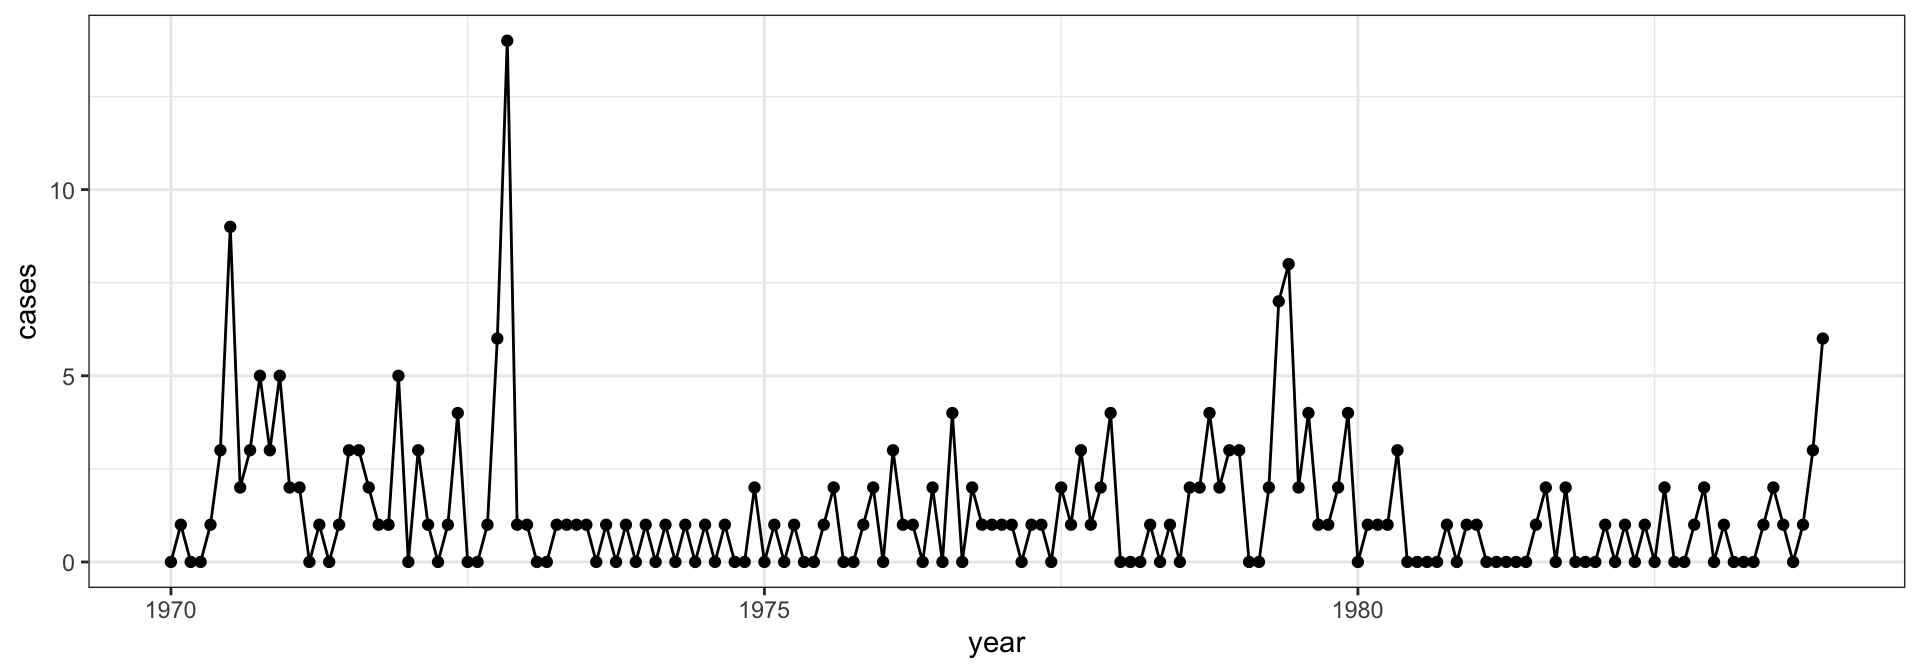
\includegraphics[width=0.6\textwidth]{Lec17_files/figure-beamer/unnamed-chunk-11-1} \end{center}

\pause

\[
\symbf{W} = \begin{pmatrix}
0 & 1 & 0 \\
1 & 0 & 1 \\
0 & 1 & 0 
\end{pmatrix}
\qquad\qquad
\symbf{D} = \begin{pmatrix}
1 & 0 & 0 \\
0 & 2 & 0 \\
0 & 0 & 1 
\end{pmatrix}
\] . . .

\[
\symbf{\Sigma} = \sigma^2 \, (\symbf{D} - \phi \, \symbf{W}) = \sigma^2~\begin{pmatrix}
1 & -\phi & 0 \\
-\phi & 2 & -\phi \\
0 & -\phi & 1 
\end{pmatrix}^{-1}
\]

\end{frame}

\begin{frame}[fragile,t]{When does \(\Sigma\) exist?}
\protect\hypertarget{when-does-sigma-exist}{}

\begin{Shaded}
\begin{Highlighting}[]
\NormalTok{check_sigma =}\StringTok{ }\ControlFlowTok{function}\NormalTok{(phi) \{}
\NormalTok{  Sigma_inv =}\StringTok{ }\KeywordTok{matrix}\NormalTok{(}\KeywordTok{c}\NormalTok{(}\DecValTok{1}\NormalTok{,}\OperatorTok{-}\NormalTok{phi,}\DecValTok{0}\NormalTok{,}\OperatorTok{-}\NormalTok{phi,}\DecValTok{2}\NormalTok{,}\OperatorTok{-}\NormalTok{phi,}\DecValTok{0}\NormalTok{,}\OperatorTok{-}\NormalTok{phi,}\DecValTok{1}\NormalTok{), }\DataTypeTok{ncol=}\DecValTok{3}\NormalTok{, }\DataTypeTok{byrow=}\OtherTok{TRUE}\NormalTok{) }
  \KeywordTok{solve}\NormalTok{(Sigma_inv)}
\NormalTok{\}}

\KeywordTok{check_sigma}\NormalTok{(}\DataTypeTok{phi=}\DecValTok{0}\NormalTok{)}
\CommentTok{##      [,1] [,2] [,3]}
\CommentTok{## [1,]    1  0.0    0}
\CommentTok{## [2,]    0  0.5    0}
\CommentTok{## [3,]    0  0.0    1}

\KeywordTok{check_sigma}\NormalTok{(}\DataTypeTok{phi=}\FloatTok{0.5}\NormalTok{)}
\CommentTok{##           [,1]      [,2]      [,3]}
\CommentTok{## [1,] 1.1666667 0.3333333 0.1666667}
\CommentTok{## [2,] 0.3333333 0.6666667 0.3333333}
\CommentTok{## [3,] 0.1666667 0.3333333 1.1666667}

\KeywordTok{check_sigma}\NormalTok{(}\DataTypeTok{phi=}\OperatorTok{-}\FloatTok{0.6}\NormalTok{)}
\CommentTok{##          [,1]     [,2]     [,3]}
\CommentTok{## [1,]  1.28125 -0.46875  0.28125}
\CommentTok{## [2,] -0.46875  0.78125 -0.46875}
\CommentTok{## [3,]  0.28125 -0.46875  1.28125}
\end{Highlighting}
\end{Shaded}

\end{frame}

\begin{frame}[fragile]{}
\protect\hypertarget{section-2}{}

\begin{Shaded}
\begin{Highlighting}[]
\KeywordTok{check_sigma}\NormalTok{(}\DataTypeTok{phi=}\DecValTok{1}\NormalTok{)}
\CommentTok{## Error in solve.default(Sigma_inv): Lapack routine dgesv: system is exactly singular: U[3,3] = 0}

\KeywordTok{check_sigma}\NormalTok{(}\DataTypeTok{phi=}\OperatorTok{-}\DecValTok{1}\NormalTok{)}
\CommentTok{## Error in solve.default(Sigma_inv): Lapack routine dgesv: system is exactly singular: U[3,3] = 0}

\KeywordTok{check_sigma}\NormalTok{(}\DataTypeTok{phi=}\FloatTok{1.2}\NormalTok{)}
\CommentTok{##            [,1]      [,2]       [,3]}
\CommentTok{## [1,] -0.6363636 -1.363636 -1.6363636}
\CommentTok{## [2,] -1.3636364 -1.136364 -1.3636364}
\CommentTok{## [3,] -1.6363636 -1.363636 -0.6363636}

\KeywordTok{check_sigma}\NormalTok{(}\DataTypeTok{phi=}\OperatorTok{-}\FloatTok{1.2}\NormalTok{)}
\CommentTok{##            [,1]      [,2]       [,3]}
\CommentTok{## [1,] -0.6363636  1.363636 -1.6363636}
\CommentTok{## [2,]  1.3636364 -1.136364  1.3636364}
\CommentTok{## [3,] -1.6363636  1.363636 -0.6363636}
\end{Highlighting}
\end{Shaded}

\end{frame}

\begin{frame}[fragile,t]{When is \(\Sigma\) positive semidefinite?}
\protect\hypertarget{when-is-sigma-positive-semidefinite}{}

\begin{Shaded}
\begin{Highlighting}[]
\NormalTok{check_sigma_pd =}\StringTok{ }\ControlFlowTok{function}\NormalTok{(phi) \{}
\NormalTok{  Sigma_inv =}\StringTok{ }\KeywordTok{matrix}\NormalTok{(}\KeywordTok{c}\NormalTok{(}\DecValTok{1}\NormalTok{,}\OperatorTok{-}\NormalTok{phi,}\DecValTok{0}\NormalTok{,}\OperatorTok{-}\NormalTok{phi,}\DecValTok{2}\NormalTok{,}\OperatorTok{-}\NormalTok{phi,}\DecValTok{0}\NormalTok{,}\OperatorTok{-}\NormalTok{phi,}\DecValTok{1}\NormalTok{), }\DataTypeTok{ncol=}\DecValTok{3}\NormalTok{, }\DataTypeTok{byrow=}\OtherTok{TRUE}\NormalTok{) }
  \KeywordTok{chol}\NormalTok{(}\KeywordTok{solve}\NormalTok{(Sigma_inv))}
\NormalTok{\}}

\KeywordTok{check_sigma_pd}\NormalTok{(}\DataTypeTok{phi=}\DecValTok{0}\NormalTok{)}
\CommentTok{##      [,1]      [,2] [,3]}
\CommentTok{## [1,]    1 0.0000000    0}
\CommentTok{## [2,]    0 0.7071068    0}
\CommentTok{## [3,]    0 0.0000000    1}

\KeywordTok{check_sigma_pd}\NormalTok{(}\DataTypeTok{phi=}\FloatTok{0.5}\NormalTok{)}
\CommentTok{##          [,1]      [,2]      [,3]}
\CommentTok{## [1,] 1.080123 0.3086067 0.1543033}
\CommentTok{## [2,] 0.000000 0.7559289 0.3779645}
\CommentTok{## [3,] 0.000000 0.0000000 1.0000000}

\KeywordTok{check_sigma_pd}\NormalTok{(}\DataTypeTok{phi=}\OperatorTok{-}\FloatTok{0.6}\NormalTok{)}
\CommentTok{##          [,1]       [,2]       [,3]}
\CommentTok{## [1,] 1.131923 -0.4141182  0.2484709}
\CommentTok{## [2,] 0.000000  0.7808688 -0.4685213}
\CommentTok{## [3,] 0.000000  0.0000000  1.0000000}
\end{Highlighting}
\end{Shaded}

\end{frame}

\begin{frame}[fragile]{}
\protect\hypertarget{section-3}{}

\begin{Shaded}
\begin{Highlighting}[]
\KeywordTok{check_sigma_pd}\NormalTok{(}\DataTypeTok{phi=}\DecValTok{1}\NormalTok{)}
\CommentTok{## Error in solve.default(Sigma_inv): Lapack routine dgesv: system is exactly singular: U[3,3] = 0}

\KeywordTok{check_sigma_pd}\NormalTok{(}\DataTypeTok{phi=}\OperatorTok{-}\DecValTok{1}\NormalTok{)}
\CommentTok{## Error in solve.default(Sigma_inv): Lapack routine dgesv: system is exactly singular: U[3,3] = 0}

\KeywordTok{check_sigma_pd}\NormalTok{(}\DataTypeTok{phi=}\FloatTok{1.2}\NormalTok{)}
\CommentTok{## Error in chol.default(solve(Sigma_inv)): the leading minor of order 1 is not positive definite}

\KeywordTok{check_sigma_pd}\NormalTok{(}\DataTypeTok{phi=}\OperatorTok{-}\FloatTok{1.2}\NormalTok{)}
\CommentTok{## Error in chol.default(solve(Sigma_inv)): the leading minor of order 1 is not positive definite}
\end{Highlighting}
\end{Shaded}

\end{frame}

\begin{frame}[t]{Conclusions}
\protect\hypertarget{conclusions}{}

Generally speaking just like the AR(1) model for time series we require
that \(|\phi| < 1\) for the CAR model to be proper.

\vspace{4mm}

These results for \(\phi\) also apply in the context where
\(\sigma^2_i\) is constant across locations (i.e.
\(\symbf{\Sigma} = (\sigma^2 \, (\symbf{I}-\phi \symbf{D}^{-1}\symbf{W}))^{-1}\))

\vspace{8mm}

As a side note, the special case where \(\phi=1\) is known as an
intrinsic autoregressive (IAR) model and they are popular as an
\emph{improper} prior for spatial random effects. An additional sum
constraint is necessary for identifiability
(\(\sum_{i=1}^n y(s_i) = 0\)).

\end{frame}

\end{document}
